
%==========================================================================

\chapter{Getting Started}
\label{Getting Started}

Before coding:

\begin{enumerate}

\item
{\bf Choose a conceptual interface (see Sections
\ref{What are conceptual interfaces} and
\ref{Which conceptual interface should I use}.}
Generally, the choice is fairly obvious.  A structured grid interface
is clearly inappropriate for an unstructured grid application.  It is
desirable to use a more specific interface if appropriate, e.g., the
linear-algebraic interface is usable from any type of grid but will
involve much more user work and prevent access to some
grid-type-specific preconditioners.

\item 
{\bf Choose your desired solver strategy. } For the typical user, this
will mean a single Krylov method and a single preconditioner.

\item 
{\bf Look up matrix requirements for each solver and preconditioner.}
Each specific solver and preconditioner has requirements from the
input matrix. This information is provided in several places:
\ref{solvers}, \hypre{} Reference Manual, and header files).

\item 
{\bf Choose a matrix class that is compatible with your solvers and
preconditioners and your conceptual interface.}

\end{enumerate}
Once the previous decisions have been made, it is time to code your
application to call \hypre{}:
\begin{enumerate}

\item
{\bf Build any necessary auxiliary structures for your chosen
conceptual interface.} This includes, e.g., the grid and stencil
structures for the structured grid interface.

\item
{\bf Build the matrix and vectors through your chosen conceptual
interface.} Each conceptual interface provides a series of calls for
entering information about your problem into
\hypre{}.

\item
{\bf Build solvers and preconditioners by giving them the input
matrix.}

\item
{\bf Set solver parameters (this is optional).}  Some parameters like
convergence tolerance are the same across solvers, while others are
solver specific.

\item
{\bf Call the solve function for the solver.}

\item
{\bf Retrieve desired information from solver.} Depending on your
application, there may be different things you may want to do with the
solution vector. Also, performance information such as number of
iterations is typically available, though it may differ from solver to
solver.

\end{enumerate}

%==========================================================================

\section{A Simple Example}

The following code sample serves as a simple example of the usage of
\hypre{}. In this example, the structured grid interface (discussed in
Chapter ~\ref{Structured Grid Interface}) is used to enter the problem
into \hypre{}, and the \code{PFMG} Multigrid solver is used to solve
the system.

\begin{display}
\begin{verbatim}

/*-----------------------------------------------------------
 * Set up the matrix
 *-----------------------------------------------------------*/

HYPRE_StructGridCreate(MPI_COMM_WORLD, dim, &grid);
/* Use HYPRE_StructGridSetExtents to define grid indices */
HYPRE_StructGridAssemble(grid);
	
HYPRE_StructStencilCreate(dim, stencil_size, &stencil);
/* Use HYPRE_StructStencilSetElement to define the stencil shape */

HYPRE_StructMatrixCreate(MPI_COMM_WORLD, grid, stencil, &A);
HYPRE_StructMatrixInitialize(A);
/* Use HYPRE_StructMatrixSetBoxValues to set matrix coefficients */
HYPRE_StructMatrixAssemble(A);

/*-----------------------------------------------------------
 * Set up the right-hand side and initial guess
 *-----------------------------------------------------------*/

HYPRE_StructVectorCreate(MPI_COMM_WORLD, grid, &b);
HYPRE_StructVectorInitialize(b);
/* Use HYPRE_StructVectorSetBoxValues to set right-hand side values */
HYPRE_StructVectorAssemble(b);

HYPRE_StructVectorCreate(MPI_COMM_WORLD, grid, &x);
HYPRE_StructVectorInitialize(x);
/* Use HYPRE_StructVectorSetBoxValues to set initial guess values */
HYPRE_StructVectorAssemble(x);

/*-----------------------------------------------------------
 * Set up solver
 *-----------------------------------------------------------*/

HYPRE_StructPFMGCreate(MPI_COMM_WORLD, &solver);
HYPRE_StructPFMGSetMaxIter(solver, 50);  /* optional parameter */
HYPRE_StructPFMGSetTol(solver, 1.0e-06); /* optional parameter */
HYPRE_StructPFMGSetup(solver, A, b, x);

/*-----------------------------------------------------------
 * Solve the linear system
 *-----------------------------------------------------------*/

HYPRE_StructPFMGSolve(solver, A, b, x);

/*-----------------------------------------------------------
 * Get solution info
 *-----------------------------------------------------------*/

/* Use HYPRE_StructVectorGetBoxValues to get solution vector */

/*-----------------------------------------------------------
 * Free up memory
 *-----------------------------------------------------------*/

HYPRE_StructPFMGDestroy(solver);
HYPRE_StructGridDestroy(grid);
HYPRE_StructStencilDestroy(stencil);
HYPRE_StructMatrixDestroy(A);
HYPRE_StructVectorDestroy(b);
HYPRE_StructVectorDestroy(x);

\end{verbatim}
\end{display}

%==========================================================================

\section{What are conceptual interfaces?}
\label{What are conceptual interfaces}

\begin{figure}
\centering
\includegraphics[width=5in]{concep_iface.eps}
\caption{%
Graphic illustrating the notion of conceptual interfaces.
All of these elements are not necessarily in \hypre{}.}
\label{fig-conceptual-interface}
\end{figure}

The top row of Figure \ref{fig-conceptual-interface} illustrates a
number of conceptual interfaces.  Generally, the conceptual interfaces
are denoted by different types of computational grids, but other
application features might also be used, such as geometrical
information.  These conceptual interfaces are intended to represent
the way that applications developers naturally think of their linear
problem, and provide natural interfaces for them to pass the data that
defines their linear system into \hypre{}.  Essentially, these
conceptual interfaces can be considered convenient utilities for
helping a user build a matrix data structure for \hypre{} solvers and
preconditioners.  For example, applications that use structured grids
(such as in the left-most interface in the Figure
\ref{fig-conceptual-interface}) typically view their linear problems
in terms of stencils and grids.  On the other hand, applications that
use unstructured grids and finite elements typically view their linear
problems in terms of elements and element stiffness matrices.
Finally, the right-most interface is the standard linear-algebraic
(matrix rows/columns) way of viewing the linear problem.

The second row of Figure \ref{fig-conceptual-interface} is a set of
linear solver algorithms.  Each linear solver group requires different
information from the user through the conceptual interfaces.  So, the
geometric multigrid algorithm (GMG) listed in the left-most box, for
example, can only be used with the left-most conceptual interface.  On
the other hand, the ILU algorithm in the right-most box may be used
with any conceptual interface.

The third row of Figure \ref{fig-conceptual-interface} is a list of
data layouts or matrix/vector storage schemes.  The relationship
between linear solver and storage scheme is similar to that of
interface and linear solver.

%==========================================================================

\section{Which conceptual interface should I use?}
\label{Which conceptual interface should I use}

\hypre{} currently supports four conceptual interfaces:

\begin{itemize}

\item
\code{Structured Grid Interface:}
This interface is appropriate for applications whose grids consist of
unions of logically rectangular grids with a fixed stencil pattern of
nonzeros at each grid point.  Contributions to the matrix are made in
terms of the stencils.  {\bf NOTE:} The current version only supports
a single unknown per grid point.

\item
\code{Semi-Structured Grid Interface:}
This interface is appropriate for applications whose grids are mostly
structured, but with some unstructured features.  Examples include
block-structured grids, composite grids from structured adaptive mesh
refinement (AMR) applications, and overset grids.  This interface
supports multiple unknowns per cell.  {\bf NOTE:} This is a very new
interface, and should be used with caution while it matures.

\item
\code{Finite Element Interface:}
This is appropriate for users who form their linear systems from a
finite element discretization.  The interface mirrors typical finite
element data structures, including element stiffness matrices.  Though
this interface is provided in \hypre{}, its definition was determined
elsewhere (www.z.ca.sandia.gov/fei).

\item
\code{IJ interface:}
This is the traditional linear algebraic interface.  It can be used as
a last resort by users for whom the other grid-based interfaces are
not appropriate.  It requires more work on the user's part, though
still less than building parallel sparse data structures.  General
solvers and preconditioners are available through this interface, but
not specialized solvers which need more information.  Our experience
is that users with legacy codes, in which they already have code for
building matrices in particular formats, find the IJ interface
relatively easy to use.

\end{itemize}

Generally, a user should choose the most specific interface that
matches their application, because this will allow them to use
specialized and more efficient solvers and preconditioners without
losing access to more general solvers.

%==========================================================================

\section{Bug Reporting}

\hypre{} has an automated bug reporting mechanism in place that may be used 
as a resource for submitting bugs, desired features, and documentation
problems, as well as querying the status of previous reports.  Access
\htmladdnormallink{http://apollo.llnl.gov:8080/bugs}{http://apollo.llnl.gov:8080/bugs}
for full bug tracking details or to submit or query a bug report.
This website is currently available only within the llnl.gov domain.
When using the CASC bug reporting site for the first time, click on
``Open a new Bugzilla account'' under the ``User login account
management'' heading.

